\documentclass[11pt]{article}

\usepackage[utf8]{inputenc}
\usepackage[T1]{fontenc}
\usepackage{graphicx}
\usepackage{booktabs}
\usepackage{amsmath}
\usepackage{url}
\usepackage{hyperref}
\usepackage{cite}

\usepackage{color}
\renewcommand\UrlFont{\color{blue}\rmfamily}
\urlstyle{rm}

%%%% My packages
\usepackage{todonotes}
\usepackage{siunitx} 
\usepackage{pgf}
\usepackage{import}
\usepackage{lmodern}    
\def\mathdefault#1{#1}

\usepackage{epstopdf}
% Write EPS->PDF conversions into the build folder instead of next to the source.
\epstopdfsetup{outdir=build/}

%%%% Result values -- single source of truth. Update a value here and it
%%%% propagates everywhere it is referenced in the document.
% Temperature Scaling
\newcommand{\tsTemp}{1.126}             % optimal temperature
\newcommand{\tsCalibrationR}{0.539}     % mean R on calibration dataset
\newcommand{\tsTestR}{0.439}            % mean R on test dataset
% Monte Carlo Dropout
\newcommand{\mcdRate}{0.003}            % optimal dropout rate
\newcommand{\mcdCalibrationR}{0.464}    % mean R on calibration dataset
\newcommand{\mcdTestR}{0.469}           % mean R on test dataset
% Levenshtein Monte Carlo Dropout
\newcommand{\lmcdRate}{0.037}           % optimal dropout rate
\newcommand{\lmcdCalibrationR}{0.716}   % mean R on calibration dataset
\newcommand{\lmcdTestR}{0.679}          % mean R on test dataset

\usepackage[acronym]{glossaries}
\makeglossaries

\newacronym{ts}{TS}{Temperature Scaling}
\newacronym{mcd}{MCD}{Monte Carlo Dropout}
\newacronym{lmcd}{LMCD}{Levenshtein Monte Carlo Dropout}
\newacronym{cmaes}{CMA-ES}{Covariance Matrix Adaptation Evolution Strategy}

\newacronym{wer}{WER}{Word Error Rate}


\newacronym{ue}{UE}{Uncertainty Estimation}
\newacronym{uq}{UQ}{Uncertainty Quantification}
\newacronym{asr}{ASR}{Automatic Speech Recognition}
\newacronym{ai}{AI}{Artificial Intelligence}

\newacronym{ciempiess}{CIEMPIESS}{Corpus de Investigación en Español de México del Posgrado de Ingeniería Eléctrica y Servicio Social}

%%
%% end of the preamble, start of the body of the document source.
\begin{document}

\title{\acrshort{cmaes} for Hyperparameter Optimization of Sequence-level Uncertainty Quantification Techniques for \acrshort{asr}}

\author{
    Erick Alejandro Muñoz-Alvarado\thanks{Instituto Tecnológico de Costa Rica, Cartago, Costa Rica. \texttt{erickmatec@estudiantec.cr}}
    \and
    Saúl Calderón Ramírez\thanks{Instituto Tecnológico de Costa Rica, Cartago, Costa Rica.}
}

\date{}

\maketitle

%%
%% The abstract is a short summary of the work to be presented in the
%% article.
\begin{abstract}
    As \acrshort{ai} deployments move from lab environments into our day to day lives and safety-critical applications, the need for robust \acrshort{uq} methods becomes less of a commodity and more of a requirement. In this work, we investigate the use of \acrfull{cmaes} to optimize the hyperparameters of three \acrshort{uq} methods, \acrfull{ts}, \acrfull{mcd} and a Levenshtein-based \acrshort{mcd} variation, all of them applied to OpenAI's Whisper models for Spanish speech transcription. We evaluate each method's ability to produce uncertainty scores that represent actual transcription errors by measuring Pearson correlation between the scores and the \acrlong{wer} of the transcription. We demonstrate that \acrshort{cmaes} effectively navigates the hyperparameter landscape, yielding substantial improvements in calibration quality for each method. Our results show that \acrfull{lmcd} significantly outperforms hyperparameter tunned \acrshort{ts} and \acrshort{mcd}. Notably, \acrshort{cmaes} optimization revealed that both \acrshort{mcd} and \acrshort{lmcd} require extremely low dropout rates to provide meaningful uncertainty estimates, while \acrshort{ts} provided similar results across multiple temperature values.
\end{abstract}

\noindent\textbf{Keywords:} Uncertainty, Speech-to-Text, Temperature Scaling, Dropout, Transformers, Levenshtein

\listoftodos
\section{Introduction}

\acrfull{asr} systems have achieved remarkable performance in recent years, driven by large-scale pretrained models such as OpenAI's Whisper \cite{radford2023robust}. These models, particularly when fine-tuned for specific languages and domains, can produce transcriptions with 3\% \acrfull{wer} and in some cases even less as measured by \cite{srivastav2025open}. However, in safety-critical applications like medical dictation, legal transcription, and autonomous systems, knowing when a model is likely to make a mistake is just as important as the quality of the transcription itself\cite{koenecke2024careless}. This motivates the need for reliable \acrfull{ue} methods that can flag potential errors on each transcription.

Several approaches have been proposed for estimating predictive uncertainty in deep learning models. \acrfull{ts} \cite{guo2017calibration} adjusts the softmax distribution's sharpness via a single scalar parameter, providing a lightweight post-hoc calibration method. \acrfull{mcd} \cite{gal2016dropout} leverages dropout at inference time to approximate Bayesian inference, generating a distribution of predictions whose variance serves as an uncertainty estimate. Similar work has used \acrshort{mcd}-based implementations to estimate uncertainty and craft adversarial attacks on ASR systems \cite{jayashankar2020detecting}.
We build upon the ideas proposed by \cite{rodriguez2024uncertainty} with the use of a modification to \acrshort{mcd} where the uncertainty score is not the variance of the predictions but the Levenshtein distance between the centroid and the other predictions, which we call \acrfull{lmcd}.

While these methods have shown promise, a critical yet often overlooked challenge in deploying them is hyperparameter selection, the temperature in \acrshort{ts} and the dropout rate in \acrshort{mcd} dramatically affect the quality of the uncertainty estimates. Grid search and manual tuning are commonly employed but may miss optimal configurations. Moreover, the objective function for maximizing the correlation between uncertainty scores and actual errors is non-differentiable, noisy, and expensive to evaluate.

\acrfull{cmaes} \cite{hansen2001completely} is a derivative-free optimization algorithm particularly suited to such problems. It maintains a multivariate normal distribution over the search space and adapts both its mean and covariance matrix based on the fitness of sampled candidate solutions, making it robust to noise, non-convexity, and ill-conditioning. \acrshort{cmaes} has been successfully applied to hyperparameter optimization in various machine learning contexts \cite{loshchilov2016cma}\cite{Feurer2019}, but its application to sequence-level \acrshort{uq} hyperparameter tuning in ASR remains unexplored.

We formalize the \acrshort{uq} hyperparameter optimization problem for ASR as a black-box optimization task and apply \acrshort{cmaes} to solve it for \acrshort{ts}, \acrshort{mcd}, and \acrshort{lmcd}.
We conduct a comprehensive 10-fold cross-validation evaluation on the SpaTrans\footnote{\UrlFont{https://huggingface.co/datasets/saul1917/SpaTrans\_UQ\_Bench\_raw.}} \acrshort{uq} Bench dataset.
We demonstrate that \acrshort{cmaes} discovers non-trivial optimal hyperparameter configurations particularly for \acrshort{lmcd}.

\section{Experiment design}

\subsection{Data}

To guarantee the diversity of data, we leveraged \acrfull{ciempiess}\cite{hernandez2017automatic}, a Spanish corpus with Mexican accent, to build a subsample of 205 audios, all of them were manually revised to correct and validate the transcriptions. This curated sample consists of \qty{26}{\minute} and \qty{49}{\second} of speech.
We also used the Google Chilean dataset \cite{guevara-rukoz-etal-2020-crowdsourcing}, this included a total of \qty{7}{\hour} of curated conversations in Spanish with Chilean accent, in this case we also sampled 395 audios for a total of \qty{39}{\minute} and \qty{11}{\second} of speech.

We concatenated both datasets to obtain a total of 600 audios, stored at \qty{16}{\kilo\hertz}, the transcriptions are normalized by removing punctuation, accents, and converting all characters to lowercase. Then performed a 10-fold cross-validation split, using \qty{60}{\percent} for fine tuning, \qty{20}{\percent} for calibration of the \acrshort{uq} method (if required), and \qty{20}{\percent} for testing, ensuring that each fold contains a representative mix of both Mexican and Chilean accents.

Finally, \SI{50}{\percent} of the calibration and test datasets are contaminated with urban noise audio taken from Urban Sounds\footnote{\UrlFont{https://huggingface.co/datasets/MichielBontenbal/UrbanSounds}}. We use a linear combination of the original audio and noisy recording, with a 0.6 of weight for the noisy audio, and 0.4 for the original to contaminate the aforementioned datasets.

\subsection{Model}

OpenAI's Whisper \cite{radford2023robust} was selected as the base model for our experiments, specifically the "base" variant, which has 74 million parameters and is designed for efficient inference while maintaining strong performance. We fine-tuned the model on the fine-tune portion of each fold for 600\todo{Preguntar a daniel cuantos epoch fueron} epochs using a learning rate of 1e-5\todo{Preguntar a daniel lr} and a batch size of 16\todo{Preguntar a daniel el batch size}. The fine-tuning process was performed on an NVIDIA A100 GPU\todo{Preguntar a daniel GPU de fine tuneo}, and we monitored the training loss to ensure convergence without overfitting.

\subsection{Evaluation metrics}

\subsubsection{Word Error Rate}
This will work as the primary metric for evaluating transcription quality, \acrshort{wer} measures the edit distance between the predicted transcription and the reference transcription, normalized by the number of words in the reference.

\subsubsection{Uncertainty Score}
This metric is dependent on the \acrshort{uq} method being evaluated the specifics for each method will be detailed on the following sections, but the main idea is that the uncertainty score is a scalar value that represents the model's confidence on its prediction, where higher values indicate less confidence, so in every case we want to minimize this value.

\subsubsection{Pearson Correlation Coefficient (R)}
In order to evaluate the quality of the uncertainty estimates, we compute the Pearson correlation coefficient between the uncertainty scores produced by each method and the actual \acrshort{wer} for each audio sample in the test set. A higher absolute value of the correlation coefficient indicates a stronger relationship between the uncertainty estimates and the true error rates, which is desirable for effective \acrshort{uq}.
Also, we use this metric as the objective function for optimizing hyperparameters of each \acrshort{uq} method, so that we can find the hyperparameter combination that maximizes the relationship between the uncertainty and the \acrshort{wer}.

\subsection{Uncertainty Quantification Methods}

\subsubsection{Temperature Scaling}
We use \acrshort{cmaes} to optimize the temperature parameter $\tau$, which is applied as a post-processing step to the model's output logits. For each token position $t$ we divide the logits $z_t$ by $\tau$ before the softmax and keep the maximum scaled probability $p_t = \max_v \operatorname{softmax}(z_t / \tau)_v$, as an equivalent to greedy decoding. The uncertainty score is one minus the mean of these maximum probabilities across the sequence:
\begin{equation}
    u = 1 - \frac{1}{L}\sum_{t=1}^{L} p_t,
    \qquad p_t = \max_v \operatorname{softmax}(z_t / \tau)_v,
\end{equation}
where $L$ is the length of the predicted sequence. The objective function for optimization is the Pearson correlation coefficient between the scaled uncertainty scores and the actual \acrshort{wer}.

\subsubsection{Monte Carlo Dropout}
For base \acrshort{mcd}, we apply dropout at inference time and perform $T = 10$ stochastic forward passes to obtain a distribution of predictions. For each pass $i$ and token position $t$ we keep the maximum softmax probability $p_{i,t} = \max_v \operatorname{softmax}(z_{i,t})_v$, where $z_{i,t}$ are the logits for that token. The uncertainty score is the average token-level variance across the multiple passes:
\begin{equation}
    u = \frac{1}{L}\sum_{t=1}^{L} \frac{1}{T-1}\sum_{i=1}^{T}\left(p_{i,t} - \bar{p}_t\right)^2,
    \qquad \bar{p}_t = \frac{1}{T}\sum_{i=1}^{T} p_{i,t},
\end{equation}
where $L$ is the length of the longest predicted sequence.
For this implementation we run into cases where the predicted sequences have different lengths, so we pad the per-token probabilities with 0's up to $L$ before computing the variance.
We optimize the dropout rate using \acrshort{cmaes} to maximize the Pearson correlation between the variance-based uncertainty scores and the \acrshort{wer}.

\subsubsection{Levenshtein Monte Carlo Dropout}
In \acrshort{lmcd}, we also perform $T = 10$ stochastic forward passes, producing a set of transcriptions $\{s_1, \dots, s_T\}$, but instead of using variance, we compute the Levenshtein distance \cite{levenshtein1966binary} between the predictions. To do this we first define the medoid $s_m$ as the prediction with the minimum total Levenshtein distance to all other predictions:
\begin{equation}
    s_m = \operatorname*{arg\,min}_{s_i}\sum_{j=1}^{T} \operatorname{lev}(s_i, s_j).
\end{equation}
The uncertainty score is the average Levenshtein\cite{levenshtein1966binary} distance from the medoid to every prediction, each normalized by the length of the longer of the two sequences:
\begin{equation}
    u = \frac{1}{T}\sum_{i=1}^{T} \frac{\operatorname{lev}(s_m, s_i)}{\max\left(|s_m|, |s_i|\right)},
\end{equation}
where $\operatorname{lev}(\cdot, \cdot)$ is the Levenshtein distance and $|s|$ denotes the character length of sequence $s$.
We again use \acrshort{cmaes} to find the optimal dropout rate that maximizes the correlation between these distance-based uncertainty scores and the \acrshort{wer}.

\subsection{Methodology}

Optimization of the hyperparameters for each \acrshort{uq} method was performed using \acrshort{cmaes} with a population size of 4, and 5 generations for each case. The time needed to calibrate the dropout methods was the main constraint to define the population size and the number of generations, as each evaluation required running inference multiple times for each sample in the dataset, it slowed down the optimization process significantly.
The search space for the temperature parameter in \acrshort{ts} was defined as $[0.05, 2]$, while for the dropout rate in both \acrshort{mcd} and \acrshort{lmcd}, it was defined as $[0.001, 0.9]$.
The dataset used for calibration was the same one used to fine tune the models, and the evaluation of the Pearson correlation coefficient was performed on the test set for each fold.

\section{Results}

%%%%%%%%%% Calibration results %%%%%%%%%%

On figures \ref{fig:mcd_evolution_history}, \ref{fig:ts_evolution_history}, and \ref{fig:lmcd_evolution_history}, we observe the evolution of the Pearson correlation coefficient ($R$) for each \acrshort{uq} method across generations and population members during \acrshort{cmaes} optimization, each line represents a different population member (or iteration), and the shaded area indicates the range of $R$ values across the population at each generation. The color for each bar corresponds to the value of the hyperparameter being optimized.

\begin{figure}[htbp]
    \centering
    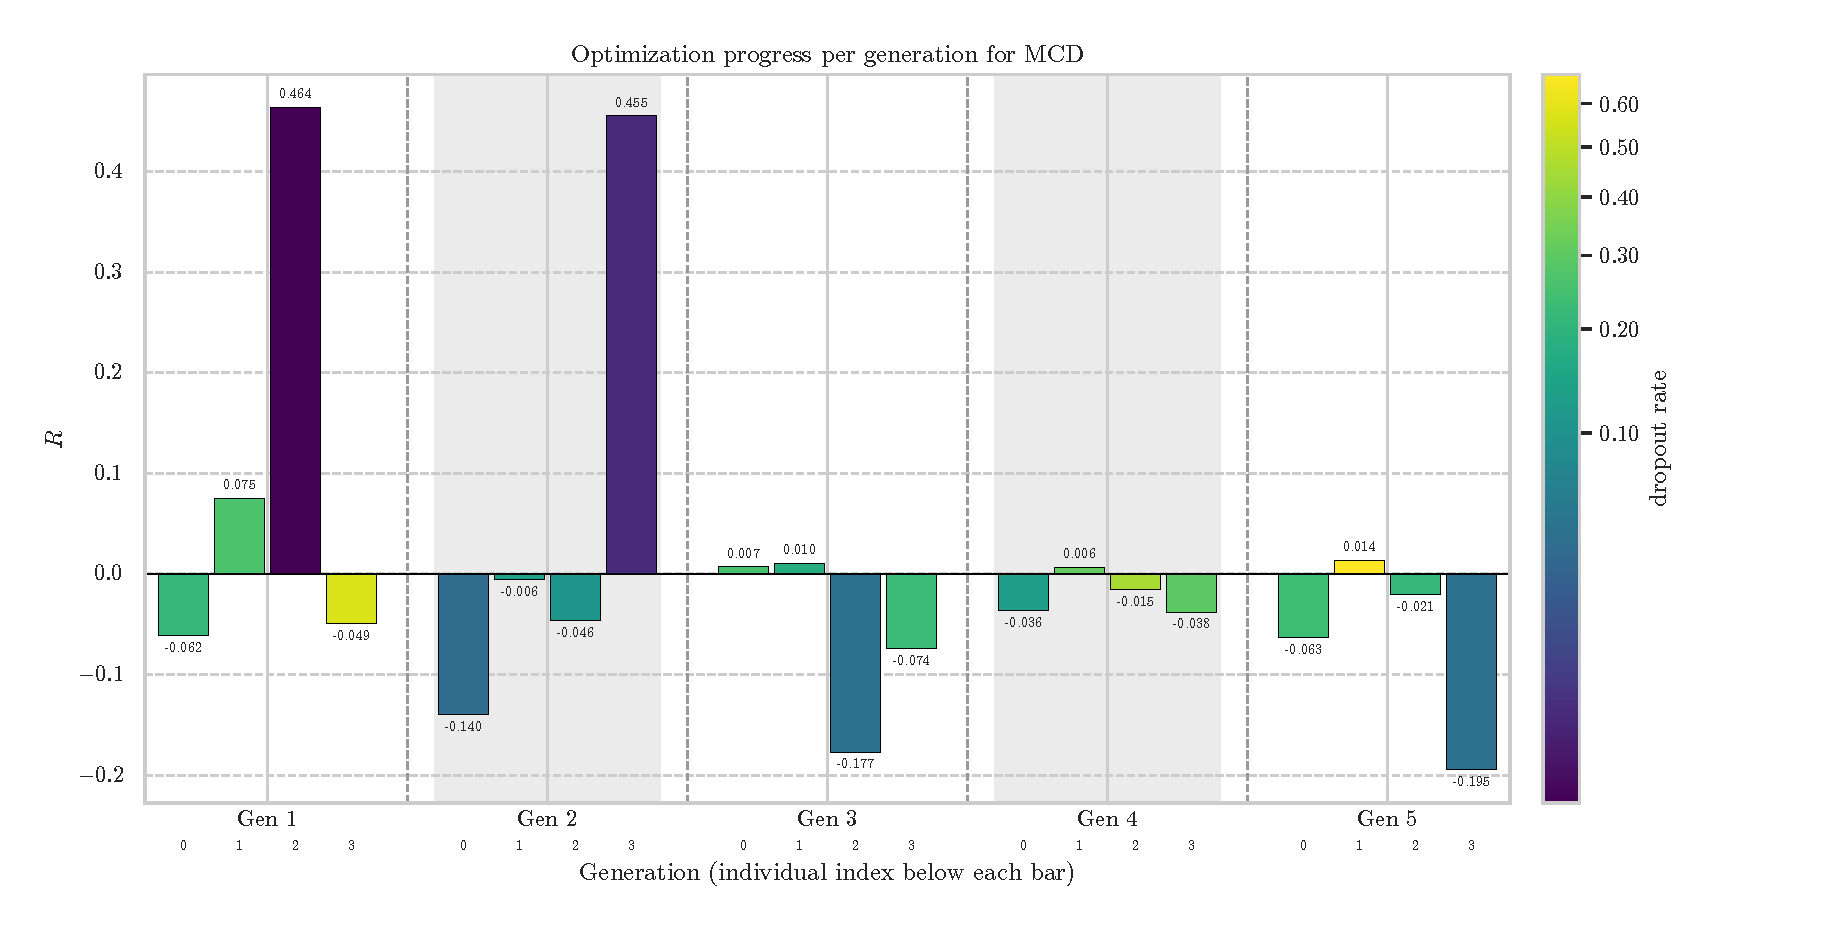
\includegraphics[width=0.9\linewidth]{imgs/mcd_evolution_history.eps}
    \caption{Evolution history of the $R$ coefficient ($R$) for the \acrshort{mcd} method.}
    \label{fig:mcd_evolution_history}
\end{figure}

\acrshort{mcd} evolution on figure \ref{fig:mcd_evolution_history} shows, the method iself is quite sensible to hyuperparameter tunning, we see that best performance on the calibration dataset is achieved with dropout rates $< 0.01$,beyond that, performance drops significantly and variance across populations increases dramatically, which suggests inestability in the optimization process, and a very narrow optimal hyperparameter range, which could be a problem for tuning this method in practice.

Best performance on the calibration dataset is achieved with a dropout rate of $\mcdRate$ and an average $R$ value of $\mcdCalibrationR$ across folds, dropout rate is much lower than the commonly used $0.1$ or $0.2$ and consistent with findings on \cite{rodriguez2024uncertainty}, this highlights the importance of careful hyperparameter tuning for \acrshort{mcd}.

\begin{figure}[htbp]
    \centering
    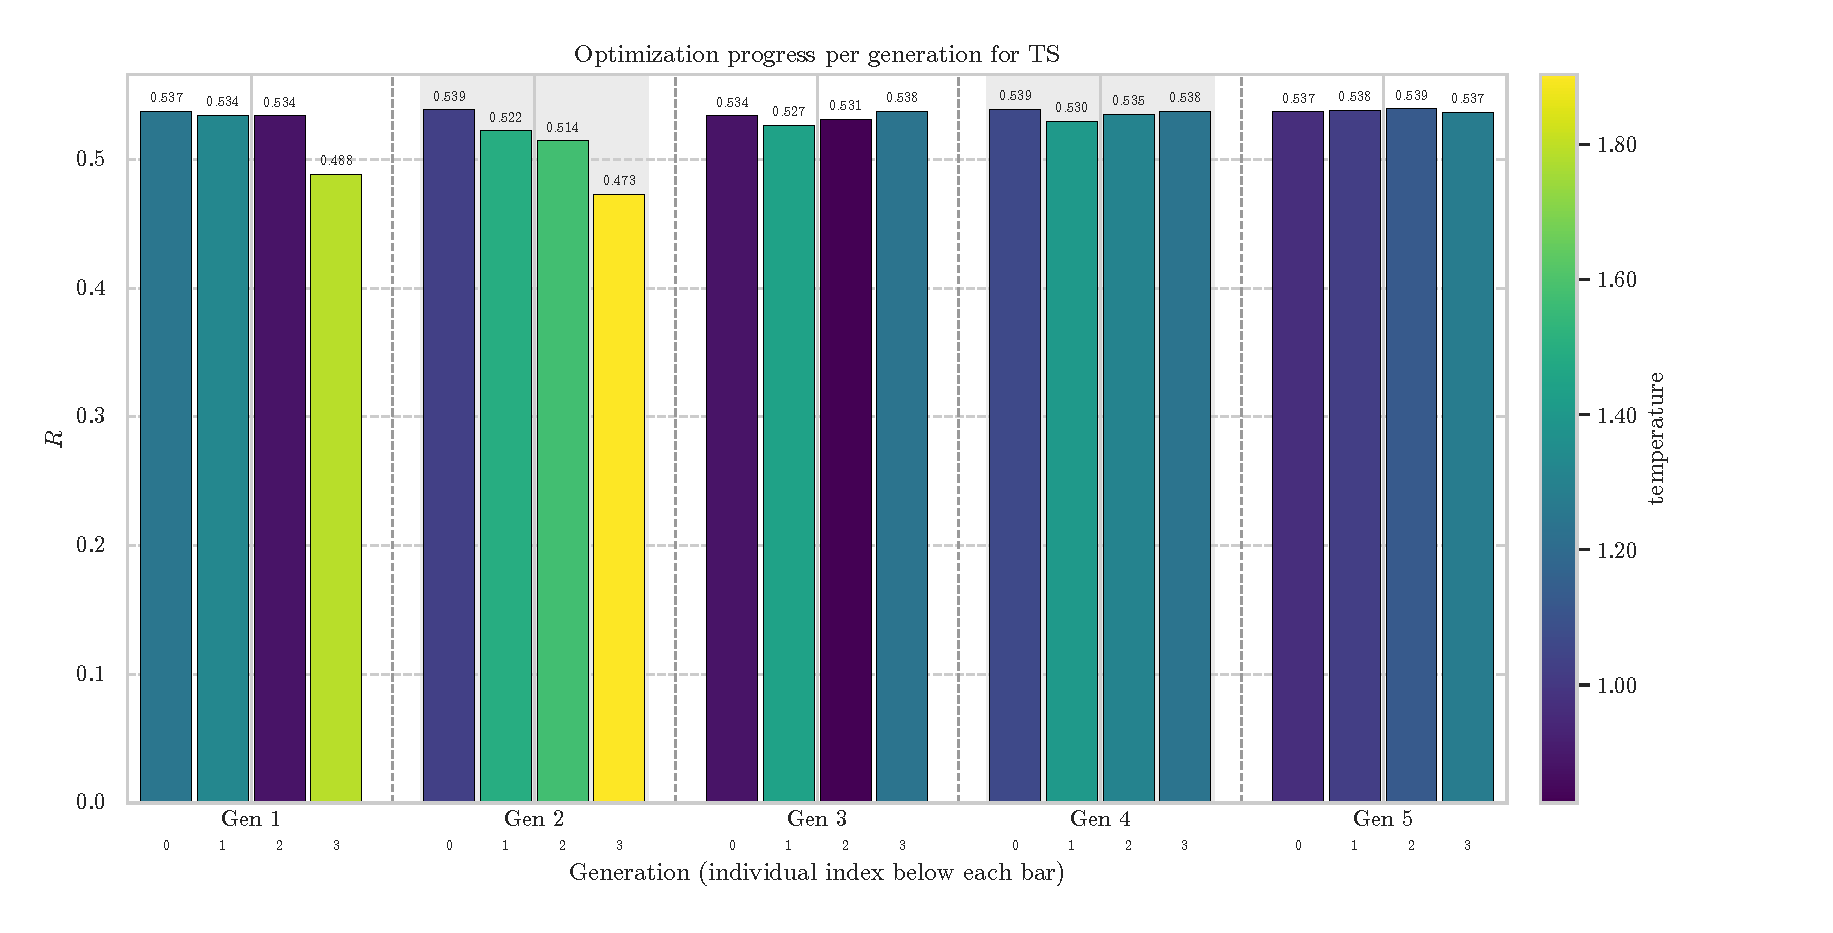
\includegraphics[width=0.9\linewidth]{imgs/ts_evolution_history.eps}
    \caption{Evolution history of the $R$ coefficient ($R$) for the \acrshort{ts} method.}
    \label{fig:ts_evolution_history}
\end{figure}

On the other hand, figure \ref{fig:ts_evolution_history} shows \acrshort{ts} is capable of providing consistent uncertainty estimates across a wide range of temperature values, with the best performance achieved around $\tau = \tsTemp$ and an average $R$ value of $\tsCalibrationR$ across folds. It's worth noting that even at the extremes performance stays stable, which suggests this method is more robust to hyperparameter selection, and could be a more practical choice when computational resources for tuning are limited.

\begin{figure}[htbp]
    \centering
    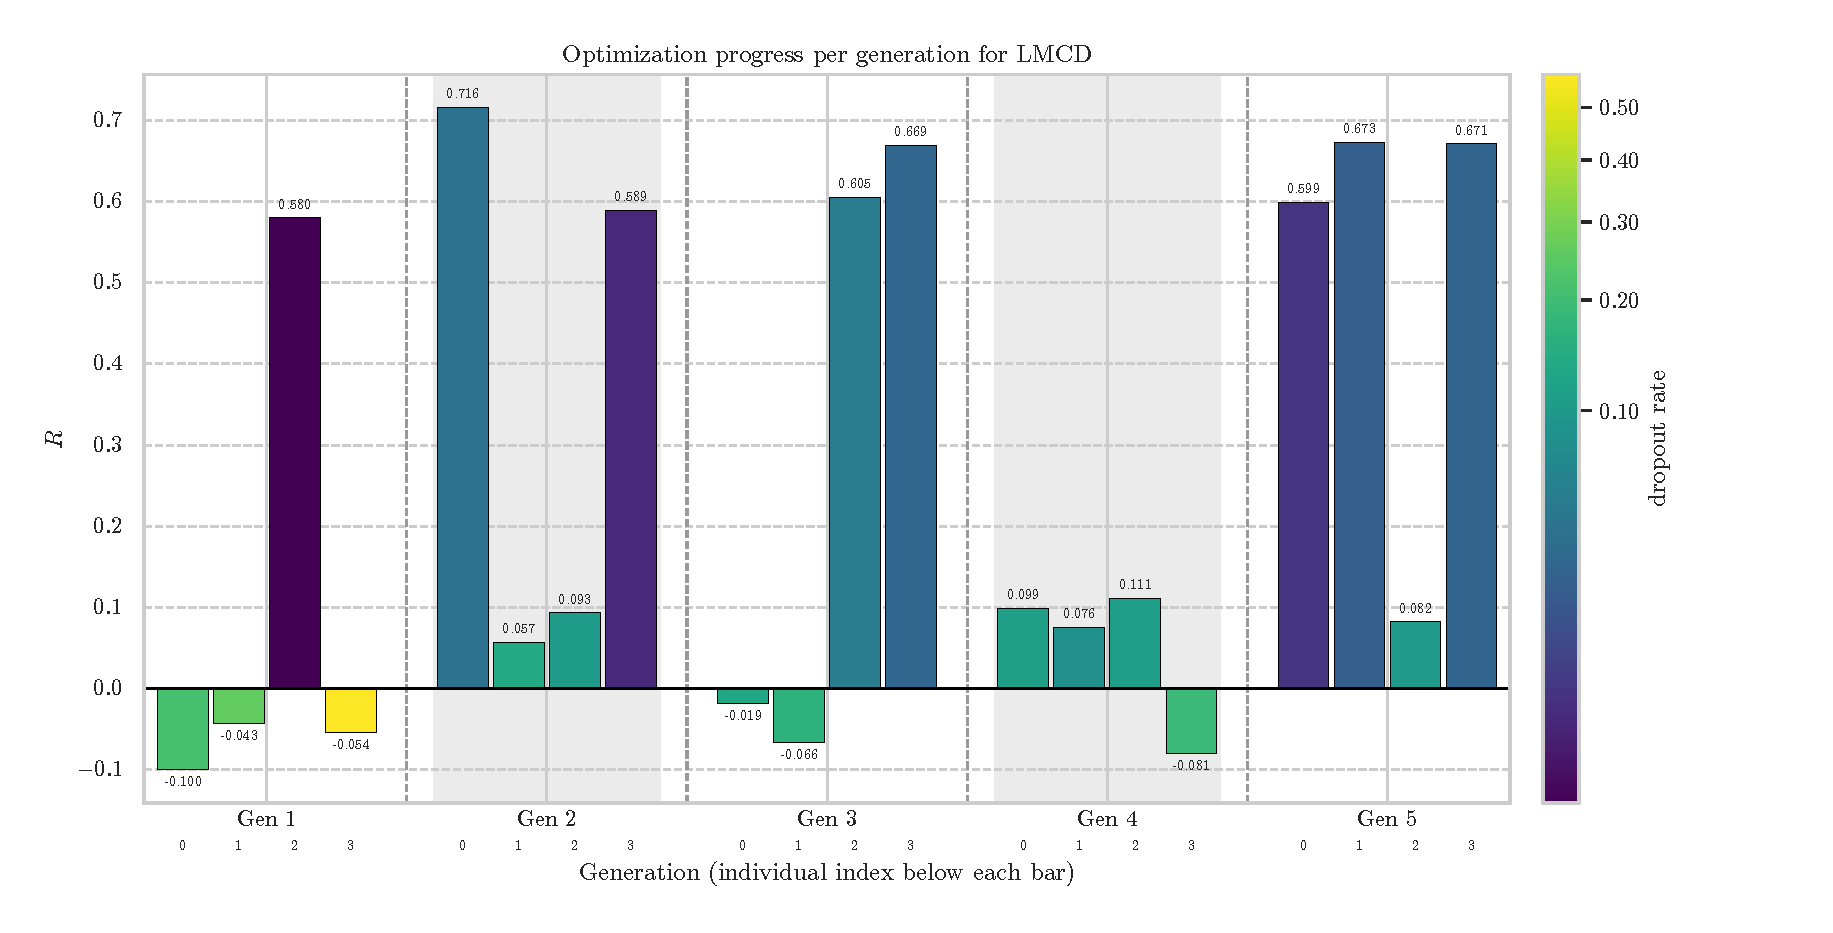
\includegraphics[width=0.9\linewidth]{imgs/lmcd_evolution_history.eps}
    \caption{Evolution history of the $R$ coefficient ($R$) for the \acrshort{lmcd} method.}
    \label{fig:lmcd_evolution_history}
\end{figure}

On figure \ref{fig:lmcd_evolution_history} \acrshort{lmcd} shows a similar pattern to \acrshort{mcd} where lower dropout ranges provide the best performance but manages to be more stable across a wider range of values. Best performance was achieved with a dropout rate of $\lmcdRate$ and an average $R$ value of $\lmcdCalibrationR$ across folds, this is where we say \acrshort{lmcd} supports the trend of lower values presenting better performance seen \acrshort{mcd}, although this is an order of magnitude higher than the best rate for \acrshort{mcd}. This could be an indication that \acrshort{lmcd} is more robust to changes in the dropout rate, which could be a significant advantage in practice, as it would make the tuning process easier and less computationally expensive while providing better performance than all the other methods.


\begin{figure}[htbp]
    \centering
    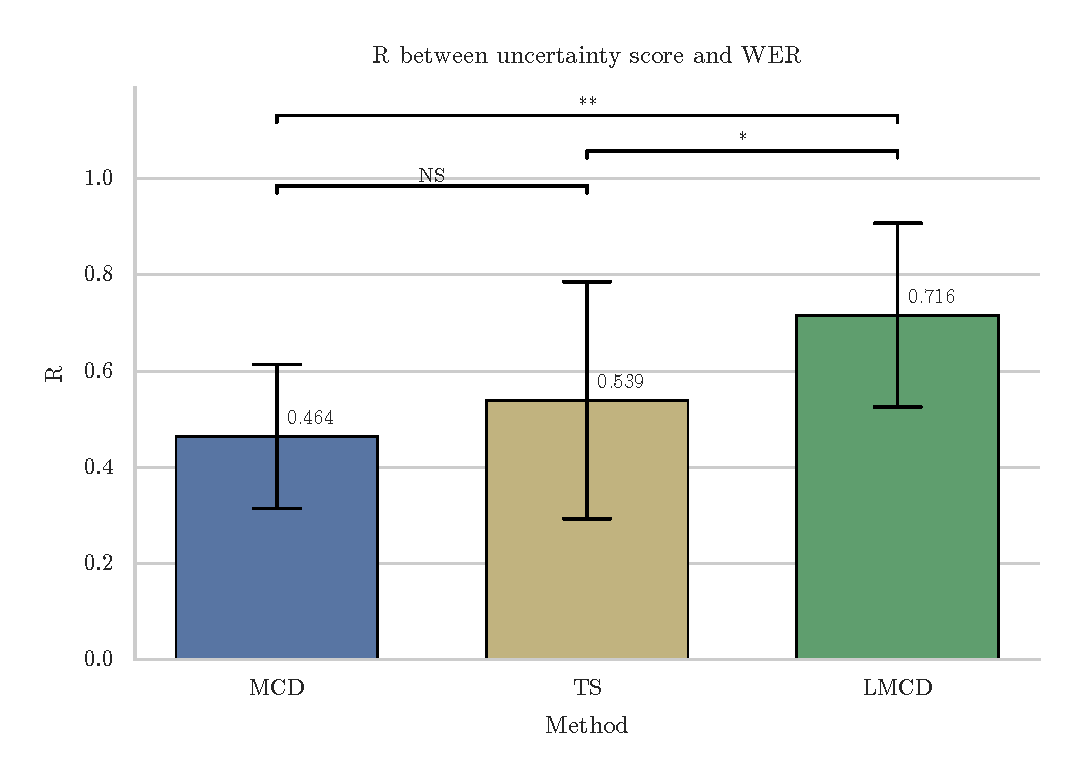
\includegraphics[width=0.9\linewidth]{imgs/best_calibration.eps}
    \caption{Best calibration results for each \acrshort{uq} method.}
    \label{fig:best_calibration_results}
\end{figure}


Table \ref{tab:wilcoxon_single_calibration} show the results of a Wilcoxon signed-rank test on the $R$ values for the best combination of hyperparameters for each method across its folds. Results show the null hypothesis can be rejected, with a p-value of $0.0009766$ and $\alpha=0.05$, which indicates that all methods provide uncertainty estimates that are statistically significant.

Figure \ref{fig:best_calibration_results} sumarizes the best calibration results for each \acrshort{uq} method, whiskers represent the standard deviation of the $R$ values across folds for that specific hyperparameter values. It also presents the results of a Paired Wilcoxon test between the methods, which shows that \acrshort{lmcd} is statistically distict to both \acrshort{mcd} and \acrshort{ts}, while \acrshort{mcd} and \acrshort{ts} are not statistically different, this suggests that the distance-based uncertainty estimation provided by \acrshort{lmcd} significantly outperforms than the variance-based estimation of \acrshort{mcd} and the post-hoc calibration of \acrshort{ts}.


\begin{table}[h]
    \centering
    \resizebox{\textwidth}{!}{%
        \begin{tabular}{|l|l|l|l|l|}
            \hline
            Method          & N  & Median & p-value   & Verdict     \\ \hline
            \acrshort{mcd}  & 10 & 0.5068 & 0.0009766 & Significant \\ \hline
            \acrshort{ts}   & 10 & 0.6634 & 0.0009766 & Significant \\ \hline
            \acrshort{lmcd} & 10 & 0.7965 & 0.0009766 & Significant \\ \hline
        \end{tabular}%
    }
    \caption{Wilcoxon signed-rank test for calibration dataset}
    \label{tab:wilcoxon_single_calibration}
\end{table}




%%%%%%%%%% Test results %%%%%%%%%%

Having defined the best hyperparameters for each method, and having validated that each one of them produces statistically significant results on the calibration dataset, we can move on to evaluate the performance of these parameters on the test dataset.

Table \ref{tab:wilcoxon_single_test} shows the results of a Wilcoxon signed-rank test on the $R$ values for the best combination of hyperparameters for each method across its folds on the test dataset. Results show the null hypothesis can be rejected for all methods and we can assert they provide uncertainty estimates that are statistically significant on the test dataset as well.

\begin{table}[]
    \centering
    \resizebox{\textwidth}{!}{%
        \begin{tabular}{|l|l|l|l|l|}
            \hline
            Method & N  & Median & P value   & Verdict     \\ \hline
            MCD    & 10 & 0.4658 & 0.0009766 & Significant \\ \hline
            TS     & 10 & 0.4262 & 0.001953  & Significant \\ \hline
            LMCD   & 10 & 0.7888 & 0.001953  & Significant \\ \hline
        \end{tabular}%
    }
    \caption{Wilcoxon signed-rank test for test dataset}
    \label{tab:wilcoxon_single_test}
\end{table}

\begin{figure}[htbp]
    \centering
    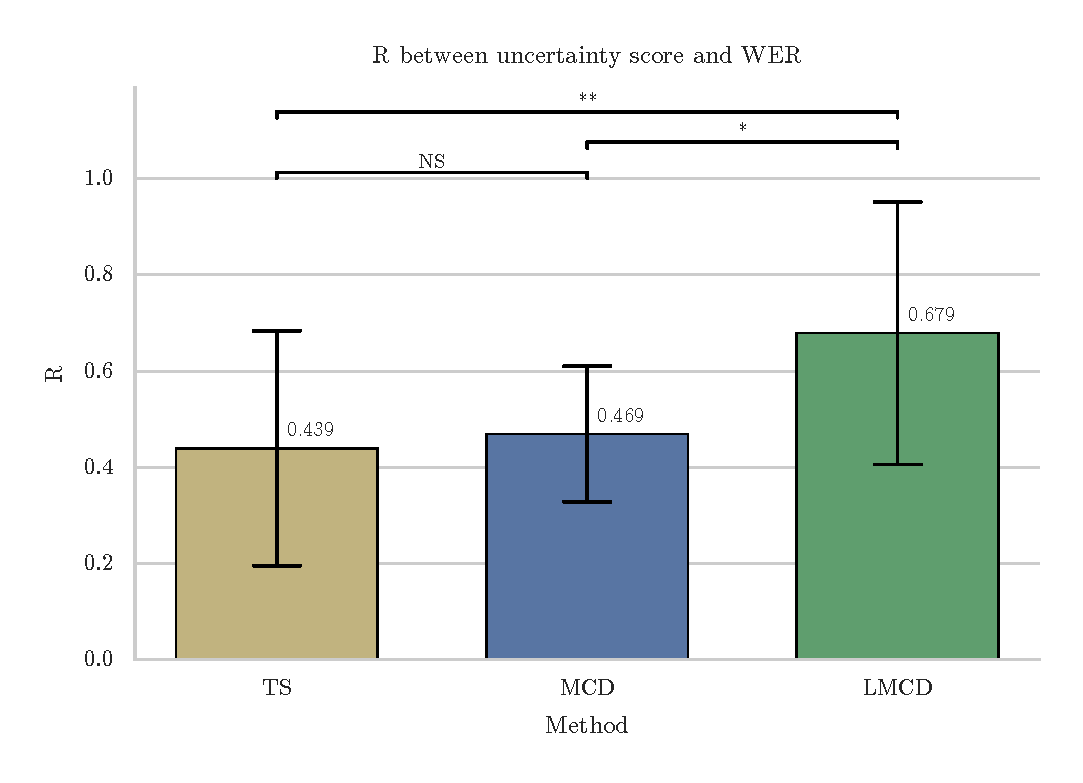
\includegraphics[width=0.9\linewidth]{imgs/best_test.eps}
    \caption{Best test results for each \acrshort{uq} method.}
    \label{fig:best_test_results}
\end{figure}


Given the results on the test dataset are statistically relevant, we move on to compare the quality of the uncertainty scores and evaluate whether the methods are statistically different from one another, to do this we perform a paired Wilcoxon signed-rank test, figure \ref{fig:best_test_results} shows that \acrshort{lmcd} is still statistically distinct to both \acrshort{mcd} and \acrshort{ts}, while \acrshort{mcd} and \acrshort{ts} are not statistically different.

By this point, we have enough data to assert that \acrshort{lmcd} is the best method for uncertainty quantification in the tasks that we have evaluated, it presents an $R$ value of $\lmcdTestR$, outperforming \acrshort{mcd} with $\mcdTestR$ and \acrshort{ts} with $\tsTestR$. It also manages to stay relatively consistent across both the calibration and test datasets, which suggests this method is more robust to changes in the data distribution, which is a trait that seem to be inherited from the second place, the \acrshort{mcd} method, which demonstrates robustness to changing datasets by maintaining almost the same $R$ value on beth datasets.

Interestingly, \acrshort{ts} is the method that degrades the most, this is consistent with other findings like \cite{yu2022robust}\cite{mozafari2018attended}, that show the $\tau$ is deeply tied to the data distribution used to calibrate it, and therefore more sensitive to data shift, this could become a problem in practice if the calibration set is not representative enough of the data the model will be used on.


\section{Conclusion}

This work demonstrates that it's possible to do hyperparameter optimization for \acrshort{lmcd}, \acrshort{mcd}, and \acrshort{ts} using \acrshort{cmaes} to achieve highly correlated uncertainty scores with the actual \acrshort{wer} of the transcriptions, which is a significant step towards making these methods more practical for real-world applications.
For example allowing the \acrshort{cmaes} algorithm converge to the fact that optimal dropout rates are much lower than commonly used defaults, highlights the importance of careful hyperparameter tuning for \acrshort{uq} methods.

The optimized \acrshort{lmcd} method significantly outperformed both \acrshort{mcd} and \acrshort{ts}, suggesting that distance-based uncertainty estimation can provide more reliable confidence measures in \acrshort{asr} systems compared to traditional approaches. Although we highlight the computational cost of tunning an \acrshort{mcd}-based algorithm, as it is significantly higher than tunning something like \acrshort{ts}, altough the performance gain and robustness shown by \acrshort{lmcd} over \acrshort{ts} is significant enough to justify the cost in scenarios where accurate uncertainty estimation is critical or the computational budget is available.

Our study focused on a specific \acrshort{asr} model and language, but the insights gained regarding the sensitivity of \acrshort{uq} methods to hyperparameters and the superiority of distance-based uncertainty estimation could have broader implications for other models and tasks.
In general we believe future work could explore more efficient optimization strategies to reduce the computational burden while still effectively navigating the hyperparameter space for \acrshort{uq} methods that target non differentiable objectives like \acrshort{wer} in this case, and investigate its effectiveness in not only in \acrshort{asr} but other areas like generation and multiple languages.

%%
%% The next two lines define the bibliography style to be used, and
%% the bibliography file.
\bibliographystyle{plain}
\bibliography{refs}


\end{document}

